\documentclass[%
 aip,
% jmp,
% bmf,
% sd,
% rsi,
cp,  % Conference Proceedings
 amsmath,amssymb,%nobibnotes,
% preprint,%
 reprint,%
%author-year,%
%author-numerical,%
]{revtex4-2}

\usepackage{graphicx}% Include figure files
\usepackage{dcolumn}% Align table columns on decimal point
\usepackage{bm}% bold math
%\usepackage[mathlines]{lineno}% Enable numbering of text and display math
%\linenumbers\relax % Commence numbering lines

\usepackage[utf8]{inputenc}
\usepackage[T1]{fontenc}
%% Loads a Times-like font. You can also load
%% {newtxtext,newtxtmath}, but not {times}, 
%% {txfonts} nor {mathtpm} as these packages
%% are obsolete and have been known to cause problems.
\usepackage{mathptmx}
\usepackage{units}

\makeatletter
\def\cat@comma@active{\catcode`\,12}%
\makeatother

\begin{document}

\title{Radio Telescope Observations Of The April 8, 2024 Total Solar Eclipse At 1420MHz.}% Force line breaks with \\

\author{August Childress} % Write as First name Surname
\email[Corresponding author: ]{achildress@cub.uca.edu}
\affiliation{Department of Physics, Astronomy, and Engineering, University of Central Arkansas, Conway, AR 72035, USA}
\author{Blayne Griffin}%
\email{bgriffin13@cub.uca.edu.}
\affiliation{Department of Physics, Astronomy, and Engineering, University of Central Arkansas, Conway, AR 72035, USA}
\author{Jeremy Lusk}
\email{jlusk@uca.edu}
\affiliation{Department of Physics, Astronomy, and Engineering, University of Central Arkansas, Conway, AR 72035, USA}

\date{\today} % It is always \today, today, but any date may be explicitly specified
              % Not printed for conference proceedings

\begin{abstract}
We present radio telescope observations of the 08 April 2024 total solar eclipse from the University of Central Arkansas campus in Conway, Arkansas using a \unit[2.3]{m} SPIDER 230C parabolic radio telescope tuned to a frequency of \unit[1420]{MHz}.
Observations began approximately \unit[19]{min} before first contact and ended approximately \unit[2.5]{min} after fourth contact, continuously tracking the sun across the sky.
Our radio observations show a reduction in relative intensity from the beginning of the lightcurve to the middle of totality of approximately 70\%, indicating that the apparent size of the radio solar disk was larger than the apparent size of the moon and therefore only partially covered.
This contrasts with optical data, where the eclipse was total.
To determine the relative size of the radio solar disk, we compared our observed radio and optical data with theoretical curves where we varied the solar radius.
From our analyses, we found that the radio solar disk is approximately $R_{\mathrm{1420}} = 1.27 R_{\odot}$.
This is consistent with previously published results.
\end{abstract}

\maketitle

\section{\label{sec:introduction}Introduction}
Our goal with this project is to determine the apparent size of the sun using \unit[1420]{MHz} radio telescope observations during the April 8th, 2024 total solar eclipse.
At this frequency, the radio emission from the sun is dominated by gyroresonance emission from electrons spiraling in the sun's extended magnetic field, which make the sun appear larger in radio frequencies than at optical frequencies.

We collected data in both the optical and radio frequencies, providing a unique opportunity to compare the relative size in the optical and radio spectra.
To accomplish this, we need to determine how much of the solar disk is obscured by the moon during totality in both the optical and radio wavelengths.
We have only one source of radio lightcurve data: UCA's 2.3 meter radio telescope.
In order to compare the radio eclipse to the optical eclipse, we have two sources of optical lightcurve data: a livestream from the UCA Observatory and a broad-spectrum light sensor pointed at the sky.
We also generated theoretical lightcurves using the software \texttt{Stellarium}\cite{zotti_simulated_2020} and the JPL Horizons On-Line Ephemeris System \cite{nasa_jpl_solar_system_dynamics_group_jpl_nodate}.
Using these data, we can compare the optical and radio lightcurves to determine the relative size of the radio solar disk.


\section{\label{sec:observations}Observations}
\subsection{\label{sec:radio}The Radio Lightcurve}
Minimal cloud cover and no sustained winds on the day of the eclipse contributed to a nearly issue free radio lightcurve.
We addressed 3 sources of error in our project: A strong gust of wind pushed the telescope off target for a few seconds, an issue with the accuracy of our polar alignment, causing the telescope to be slightly off target by the end of observation, and local sources of interference.
In order for this raw data to be compared to the optical lightcurve, these errors must be addressed.
A number of data analysis methods were used to do this:
\paragraph{Linear Adjustment function}
The first step in our data analysis is to correct for the tracking error.
We found average Analog to Digital Unit (ADU) counts for the duration of time after 4th contact and average ADU counts for the same duration of time before 1st contact.
We then created a linear function that shifts the data at the end of the lightcurve upward and decreases in effect to 0 at 1st contact.
\paragraph{Smoothing}
The next step is to smooth the data.
Our choice to smooth the data came from the need to reduce noise/random spikes in the data to get a better idea of the shape of the curve.
We chose to apply a Savitzky-Golay filter to do this.
\paragraph{Normalization}
The final step is to normalize the data.
Normalization is the process by which the data of a graph is scaled by a constant such that the highest points are equal to 100, essentially making the data a percentage of its highest value.
This is done after smoothing to avoid issues with noise spikes.
Converting the ADU counts to a relative brightness makes it possible to compare with the optical lightcurves.
\\
Now that the raw data has been refined, a neat radio lightcurve of the eclipse remains.
\subsection{\label{sec:optical}The Optical Lightcurve}
We collected optical lightcurve data to compare contact times, the depth of the eclipse, and the shape of the lightcurve to our radio observations. Our two sources include a livestream lightcurve using a solar filter-equipped optical telescope, and a Vernier Light Sensor (LS-BTA) pointed straight up at the sky.
\paragraph{The Livestream Lightcurve}
The livestream lightcurve was created by grayscaling the image of the eclipse and using Otsu thresholding to only count pixels above a certain value.
To get the time for each data point, we took an image of the in-video clock at the same time we counted the pixels of the eclipse and used computer vision to recognise the characters in the clock, giving us the time at which the frame was pixel-counted.
The number of pixels of the solar disk over time can then be normalized to a relative brightness.
We compared this livestream lightcurve to a theoretical lightcurve generated by the software \texttt{Stellarium}\cite{zotti_simulated_2020}, and were happy to see that the livestream and theoretical lightcurves overlap quite well.
\paragraph{The Light Sensor Lightcurve}
The light sensor used to collect data during the solar eclipse was the Vernier Light Sensor (LS-BTA) pointed at the sky.
Dr. Todd Abel and Shane Ayotte provided the light sensor data, which we normalized to relative brightness.
Because the light sensor data had timestamps included, we used it to confirm the accuracy of our other lightcurves timings.
\\
By stacking the lightcurves, we observed that all three had a very similar shape, with heavy overlap between the theoretical and livestream lightcurves.
This implies that our lightcurves are accurate and can be used to compare with our radio lightcurve to determine the size of the sun’s radio emission.
\\
\begin{figure}
    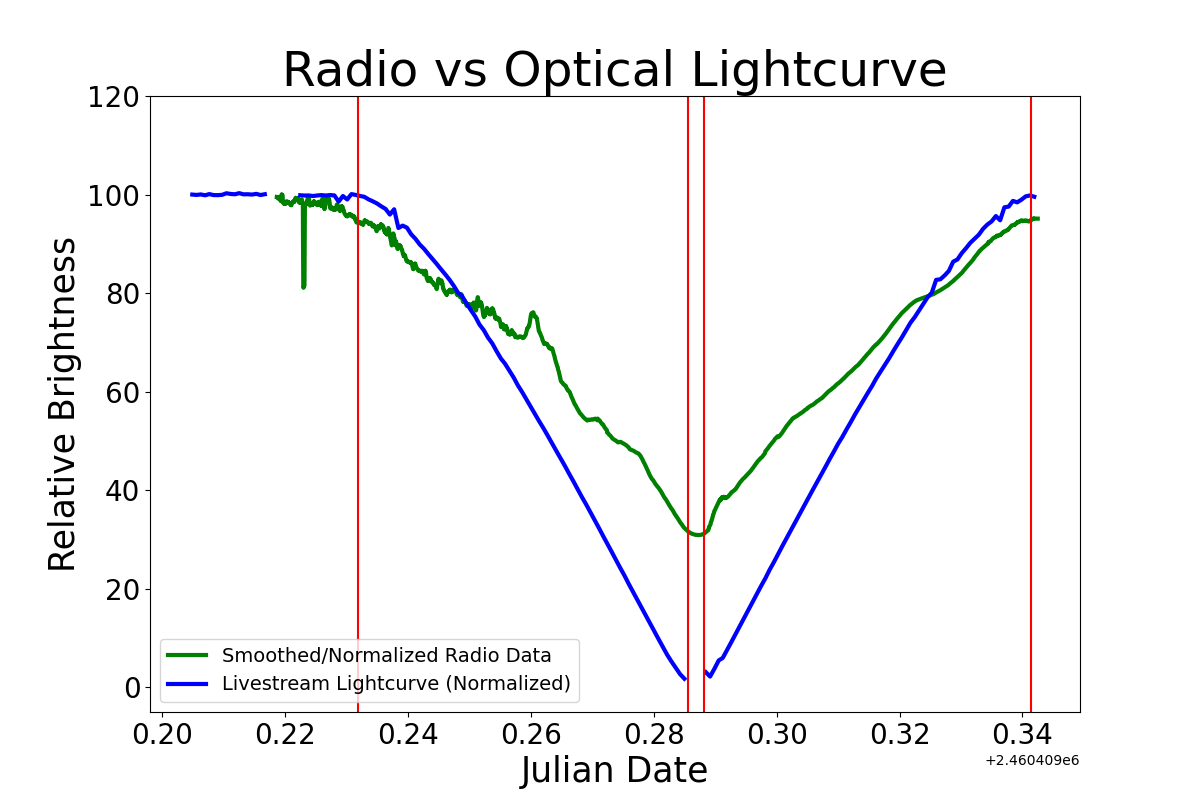
\includegraphics[width=0.5\textwidth]{figures/radioOpticalComparison}
    \caption{\label{fig:radioOpticalComparison} A comparison of the smoothed/normalized radio lightcurve and the normalized optical lightcurve generated from the livestream.}
\end{figure}

\section{\label{sec:theoretical}Theoretical Studies}
\subsection{\label{sec:stellarium}Stellarium}

\subsection{\label{sec:theoreticalLightcurves}Theoretical Lightcurve Comparison}


\section{\label{sec:conclusion}Conclusion}
Based on our comparison of data from a 2.3 m radio telescope, a broad-spectrum light sensor, an optical livestream, and theoretical data from \texttt{Stellarium} and JPL Horizons, our hypothesis that the radio solar disk is larger than the optical solar disk is supported.
This analysis found that the best-fit curve has an apparent solar radius of $R_{\mathrm{1420}} = 1.27 R_{\odot}$, falling between the results of other studies \cite{messerotti_radio_2000} and \cite{leung_solar_2022}.
In future work, we hope to examine the radio lightcurve in detail, with the goal of mapping radio emission from the sun's surface as features are eclipsed by the moon's edge moving across the face of the sun, as done in \cite{messerotti_radio_2000}.


\begin{acknowledgments}
\noindent Special thanks to these people for providing us the data necessary for our project:

% Come back and indent and make parentheses affiliations
\begin{enumerate}
    \item Scott Austin, Ph.D. (Director of Astronomical Facilities, Associate Professor of Astronomy and Physics, Department of Physics, Astronomy, and Engineering, University of Central Arkansas) 
    \item Todd Abel, Ph.D. (UCA STEM Institute Co-Director, Associate Professor of Mathematics, Secondary Mathematics Education Program Coordinator)
    \item Shane Ayotte. (UCA Mathematics Student)
\end{enumerate}

The funding to purchase the radio telescope was awarded through the Arkansas Space Grant Consortium (ASGC), grant number GR013133-22-UCA.

Support for student research funds was awarded through an ASGC Student Intensive Training grant.

\end{acknowledgments}

\nocite{*}
\bibliography{refs}% Produces the bibliography via BibTeX.

\end{document}
%
% ****** End of file aipsamp.tex ******
